% 本格式範例修改 鄭欣明教授及萬子綾同學提供之版本。本人陳昱圻僅做格式上的調整與更改。歡迎自由複製取用。
%!TEX program=xelatex
\documentclass[10pt, a4paper, twocolumn]{article}
\usepackage[margin=2.5cm]{geometry}
\setlength\columnsep{0.5cm}
\linespread{1}
\usepackage[]{authblk}

% chinese font
%\usepackage{fontspec}
\usepackage{CJKutf8}
% windows text
%\setCJKmainfont{DFKai-SB}
% overleaf or not windows environment
%\setCJKmainfont[AutoFakeBold=2,AutoFakeSlant=.4]{[kaiu.ttf]}
%\setmainfont{Times New Roman}

\usepackage{titlesec}

\titleformat{\section}
  {\fontsize{12pt}{15}\bfseries}{\thesection}{1em}{}
\titleformat{\subsection}
 {\fontsize{11pt}{15}\bfseries}{\thesubsection}{1em}{}
  \titleformat{\subsubsection}
 {\fontsize{11pt}{15}\bfseries}{\thesubsubsection}{1em}{}

\renewcommand\thesection{\arabic{section}.}
\renewcommand\thesubsection{\thesection\arabic{subsection}}
\renewcommand\thesubsubsection{\thesubsection.\arabic{subsubsection}}

\usepackage[font={bf}, labelsep=space]{caption}
\usepackage{graphicx}
\usepackage{indentfirst}
\usepackage{algorithm}
\usepackage{listings}
\usepackage[noend]{algpseudocode}
\usepackage{amsmath}
\usepackage{amssymb}
\usepackage{booktabs}
\usepackage{multicol}
\usepackage{multirow}
\usepackage{url}

\lstdefinestyle{cstyle}{
  basicstyle=\ttfamily\fontsize{7pt}{9pt}\selectfont,
  keywordstyle=\bfseries,
  frame=single,
  xleftmargin=2pt, xrightmargin=2pt,
  breaklines=true,
  captionpos=b
}
\lstdefinestyle{asmstyle}{
  basicstyle=\ttfamily\fontsize{7pt}{9pt}\selectfont,
  frame=single,
  xleftmargin=2pt, xrightmargin=2pt,
  breaklines=true,
  captionpos=b
}
\lstdefinestyle{pcodestyle}{
  basicstyle=\ttfamily\fontsize{7pt}{9pt}\selectfont,
  frame=single,
  xleftmargin=2pt, xrightmargin=2pt,
  breaklines=true,
  captionpos=b
}

\renewcommand{\abstractname}{摘要}
\renewcommand{\refname}{參考文獻}
\renewcommand{\figurename}{圖}
\renewcommand{\tablename}{表}
\renewcommand{\lstlistingname}{列表}
\makeatletter
\renewcommand{\ALG@name}{演算法}
\makeatother

% abstract
\usepackage{abstract}
\renewcommand{\abstractnamefont}{\fontsize{12pt}{15}\bfseries}
\renewcommand{\abstracttextfont}{\fontsize{10pt}{15}}
\setlength{\absleftindent}{0pt}
\setlength{\absrightindent}{0pt}

\date{}
\begin{document}
\begin{CJK*}{UTF8}{bkai}

\title{\fontsize{16pt}{1}\selectfont\textbf{基於預訓練 P-Code 表示與圖域適應之少樣本跨架構 IoT 惡意軟體分類}}

\author[1]{林禹丞}
\author[2]{鄭欣明}
\affil[ ]{台灣科技大學資訊工程系智慧型系統實驗室\textsuperscript{1, 2}}
\affil[ ]{\{m11215206、smcheng\}@mail.ntust.edu.tw\textsuperscript{1,2}}

\renewcommand{\Affilfont}{\fontsize{12pt}{1}\bfseries}
\renewcommand{\Authfont}{\fontsize{12pt}{1}\bfseries}
\renewcommand\Authand{, }
\setlength{\affilsep}{1mm}

\maketitle
\pagestyle{empty}
\thispagestyle{empty}

% ============================
% 摘要
% ============================
\begin{abstract}

物聯網（IoT）裝置廣泛運行於異質指令集架構（ISA），使得現有惡意軟體分析方法難以跨平台通用。本文提出一種以 Ghidra High P-Code 為統一中介表示之跨架構 IoT 惡意軟體偵測框架，透過結合預訓練語言模型（Pre-trained Language Model, PLM）與圖注意力網路（Graph Attention Network, GAT），同時捕捉 P-Code 指令序列之語意特徵與函式呼叫圖之結構特徵，並引入域適應（Domain Adaptation）機制，在目標架構僅有少量標記樣本的條件下縮小跨架構特徵分佈差距。實驗結果顯示，單架構場景下各架構 F1-macro 均超過 94\%；跨架構場景下，各架構交叉訓練測試的結果， F1-macro 均超過 0.88 以上，驗證本框架之有效性。

\textbf{關鍵字：}跨架構惡意軟體分析、Ghidra P-Code、預訓練語言模型、圖神經網路、域適應
\end{abstract}


% ============================
% 1. 前言
% ============================
\section{前言}

物聯網（IoT）生態系統正快速擴張，全球連網裝置數量於 2025 年已達 211 億\cite{sinha2024iot}，廣泛部署於智慧家庭、工業控制、醫療照護等場域。不同於桌機或行動裝置集中於少數指令集架構（Instruction Set Architecture, ISA），IoT 裝置橫跨 x86、ARM、MIPS、PowerPC 等異質 ISA，且普遍缺乏完善的安全防護，導致 IoT 裝置遭受的攻擊事件從 2018 年的 3,270 萬次急升至 2022 年的 1.1229 億次\cite{petrosyan2024statista}，資安威脅日益嚴峻\cite{qureshi2024systematic}。

設計 IoT 惡意軟體分析機制面臨兩項主要挑戰：第一，正因 IoT 生態系統橫跨高度異質的 ISA，惡意軟體作者得以針對同一家族同時編譯多架構版本，感染更廣泛的裝置；因此，分析方法必須具備跨架構通用性，而非僅針對單一 ISA 設計 \cite{alhanahnah2018efficient}；第二，相同的惡意行為在不同 ISA 下呈現截然不同的指令特徵，使得基於位元組序列（Byte Sequence）與操作碼（Opcode）這些特徵的方法，針對單一架構所訓練的模型無法直接遷移。更現實的困難在於，惡意軟體樣本高度集中於 x86-64 與 ARM-32 等少數主流架構，其他低資源架構幾乎無標記資料可用。基於上述挑戰，有效的跨架構惡意軟體分析需要與架構無關的特徵，如：可印字串（Printable String）、中間表示（Intermediate Representation, IR）、統計特徵。
本研究針對跨架構惡意軟體家族分析問題，以 Ghidra High P-Code 作為特徵，以預訓練語言模型（Pre-trained Language Model, PLM）對 P-Code 指令序列進行深度語意編碼、以圖注意力網路（Graph Attention Network, GAT）建模函式呼叫圖結構，並引入域適應（Domain Adaptation）機制，在目標架構僅有少量標記樣本的條件下縮小跨架構特徵分佈差距。

本研究之核心研究問題（Research Question, RQ）為：\textbf{我們該如何設計一個與架構無關（architecture-independent）的惡意軟體分析框架，使其在異質 CPU 架構（heterogeneous CPU architectures）中仍能保持高效能？}

本文之主要貢獻如下：
\begin{itemize}
  \item \textbf{架構無關特徵設計：}以 High P-Code 之操作碼序列為語意輸入，捨棄含架構相依資訊之 varnode 位址空間，並移除 Thunk 與外部函式雜訊，提升跨架構 IR 一致性；在此基礎上以 x86-64 的資料  從頭預訓練 RoBERTa 捕捉 P-Code 語意，並結合 GAT 建模函式呼叫圖之拓樸結構。
  \item \textbf{少樣本域適應：}引入圖域適應機制，在目標架構僅有每類 5 筆標記樣本的條件下，有效縮小跨架構特徵分佈差距，大幅提升遷移表現。
  \item \textbf{嚴格跨架構評估：}有別於現有研究\cite{vasan2020mthael,chaganti2022deep,ravi2022attention}將多架構混合訓練的做法，本研究明確定義訓練僅來自單一來源架構、測試來自另一目標架構的嚴格場景，並在涵蓋 ARM-32、Intel、MIPS、x86-64 之資料集上以 10 組隨機種子驗證框架有效性。
\end{itemize}


% ============================
% 2. 相關文獻
% ============================
\section{相關文獻}

% ============================
% 2.1 跨架構惡意軟體分析
% ============================
\subsection{跨架構惡意軟體分析}

在真正具備跨架構能力的特徵方面，可印字串因直接來自二進位檔案中的可讀字元序列，不依賴特定 ISA 的指令集，因此與架構無關：Lee 等人與 Cheng 等人\cite{lee2020cross,cheng2025lightweight}均以可印字串作為 IoT 惡意軟體分類特徵，驗證其在跨架構場景下的可遷移性。然而可印字串語意稀疏，且易受字串混淆攻擊影響。以平台無關 IR 為基礎的方法是另一類架構無關的特徵：CFDVex\cite{phu2019cfdvex} 以 VEX IR 結合 CFG 特徵進行跨架構 IoT 惡意軟體偵測；CIMALiR\cite{rahat2024cimalir} 以 IR 進行跨平台惡意軟體聚類；在 Assembly Code 方面，Redmond 等人\cite{redmond2018cross}最早提出以 NLP 方法學習跨架構指令嵌入，Unimap\cite{wang2023retargeted} 與 Wang 等人\cite{wang2024learning}進一步透過對比式學習遷移，在語意空間去拉近兩個架構的相似度，提升嵌入品質實現跨架構偵測。

然後目前有許多研究\cite{vasan2020mthael,chaganti2022deep,ravi2022attention}雖標榜跨架構，但實驗設置為將多個架構資料混合後共同訓練與測試，本質上仍依賴 Byte 、Opcode 序列等受架構限制之特徵，訓練時已見過各架構樣本，並非以單一來源架構訓練、另一目標架構測試的場景進行實驗。此類設置無法反映真實世界環境所面臨的挑戰，其跨架構的表現存在高估，誤導了之後的跨架構惡意軟體分析研究。

% ============================
% 2.2 中間表示與 Ghidra P-Code
% ============================
\subsection{中間表示與 Ghidra P-Code}

利用平台無關的 IR 是消除 ISA 差異的主要策略之一。CFDVex\cite{phu2019cfdvex} 以 VEX IR 為基礎，結合 CFG 特徵進行 IoT 惡意軟體偵測；CIMALiR\cite{rahat2024cimalir} 以 IR 進行跨平台 IoT 惡意軟體聚類；Greco 等人\cite{greco2025cross}以 IR 為基礎，搭配 YARA 語法產生平台無關之惡意軟體特徵碼，抵抗常見混淆技術。在二進位函式相似性分析方面，VulHawk\cite{luo2023vulhawk}、VexIR2Vec\cite{venkatakeerthy2025vexir2vec} 與 Li 等人\cite{li2025binary}分別以 IR 為核心，透過圖結構表示與嵌入學習實現跨架構函式相似性偵測。我們先前的工作\cite{lin2025cross}以 Ghidra P-Code 統計特徵分類 IoT 惡意軟體，發現單架構準確率高達 99.9\%，但跨架構場景下性能嚴重衰退，揭示純統計特徵之語意對齊局限。

Ghidra\cite{ghidra2026repo} 為 NSA 開發之開源逆向工程工具，其 P-Code\cite{ghidra2023pcode} 是一種 RTL 中間表示。P-Code 相關文獻與文檔目前仍相當有限：Naus 等人\cite{naus2022formal}為 P-Code 建立形式語意，並在此過程中發現官方文件存在多處不完整與描述不精確的問題。P-Code 分為兩層：Low P-Code 由 SLEIGH 將機器碼直接展開，保留架構特定暫存器細節；High P-Code 則由反編譯器進一步進行資料流分析（包含靜態單賦值（Static Single Assignment, SSA）轉換、死碼消除（Dead Code Elimination）、變數識別）後產生，消除架構特定細節。每條 P-Code 指令由 Varnode、Address Space 與 P-Code Operation 三部分組成，共定義 71 個操作碼，依功能分為資料搬移、控制流程、整數算術、整數比較、整數位元、浮點運算及布林與轉換等類別。如圖~\ref{fig:pcode} 所示，MIPS、ARM 與 x86-64 的 High P-Code 在同一函式下趨於一致；然而我們先前的工作\cite{lin2025cross}與 Naus 等人\cite{naus2022formal}均指出，即便在編譯器（compiler）與優化等級（optimization level）相同的條件下，相同原始碼跨架構編譯所產生的二進制檔案的 P-Code 指令序列仍存在差異；在真實世界的惡意軟體分析場景中，編譯環境更加多樣，差異只會更大，因此語意對齊仍需額外處理。本研究即以 High P-Code Operation 作為特徵，後面文字會以 P-Code 作為簡稱。


\begin{figure}[h]
\centering

\includegraphics[width=\columnwidth]{fig/high_pcode.png}
\caption{同一 C 函式在 MIPS、ARM 與 x86-64 架構下之比較}
\label{fig:pcode}
\end{figure}


% ============================
% 3. 方法
% ============================
\section{方法}

本節介紹所提方法之整體架構，包含特徵提取與前處理、預訓練語言模型、圖注意力網路與域適應四個主要模組。圖~\ref{fig:method} 為整體框架概覽，圖~\ref{fig:feature} 為特徵抽取流程。

% ============================
% 3.1 特徵提取與前處理
% ============================
\subsection{特徵提取與前處理}

本研究以 Ghidra\cite{ghidra2026repo} 對 ELF 二進位檔進行靜態分析，提取函式呼叫圖（Function Call Graph, FCG）與 High P-Code。為降低雜訊並提升跨架構一致性，過濾掉 Thunk Function 與 External Function，僅保留具實質語意的函式節點。各函式節點之 P-Code 序列作為語意輸入，函式間呼叫關係構成 FCG 的邊。

\begin{figure}[h]
\centering
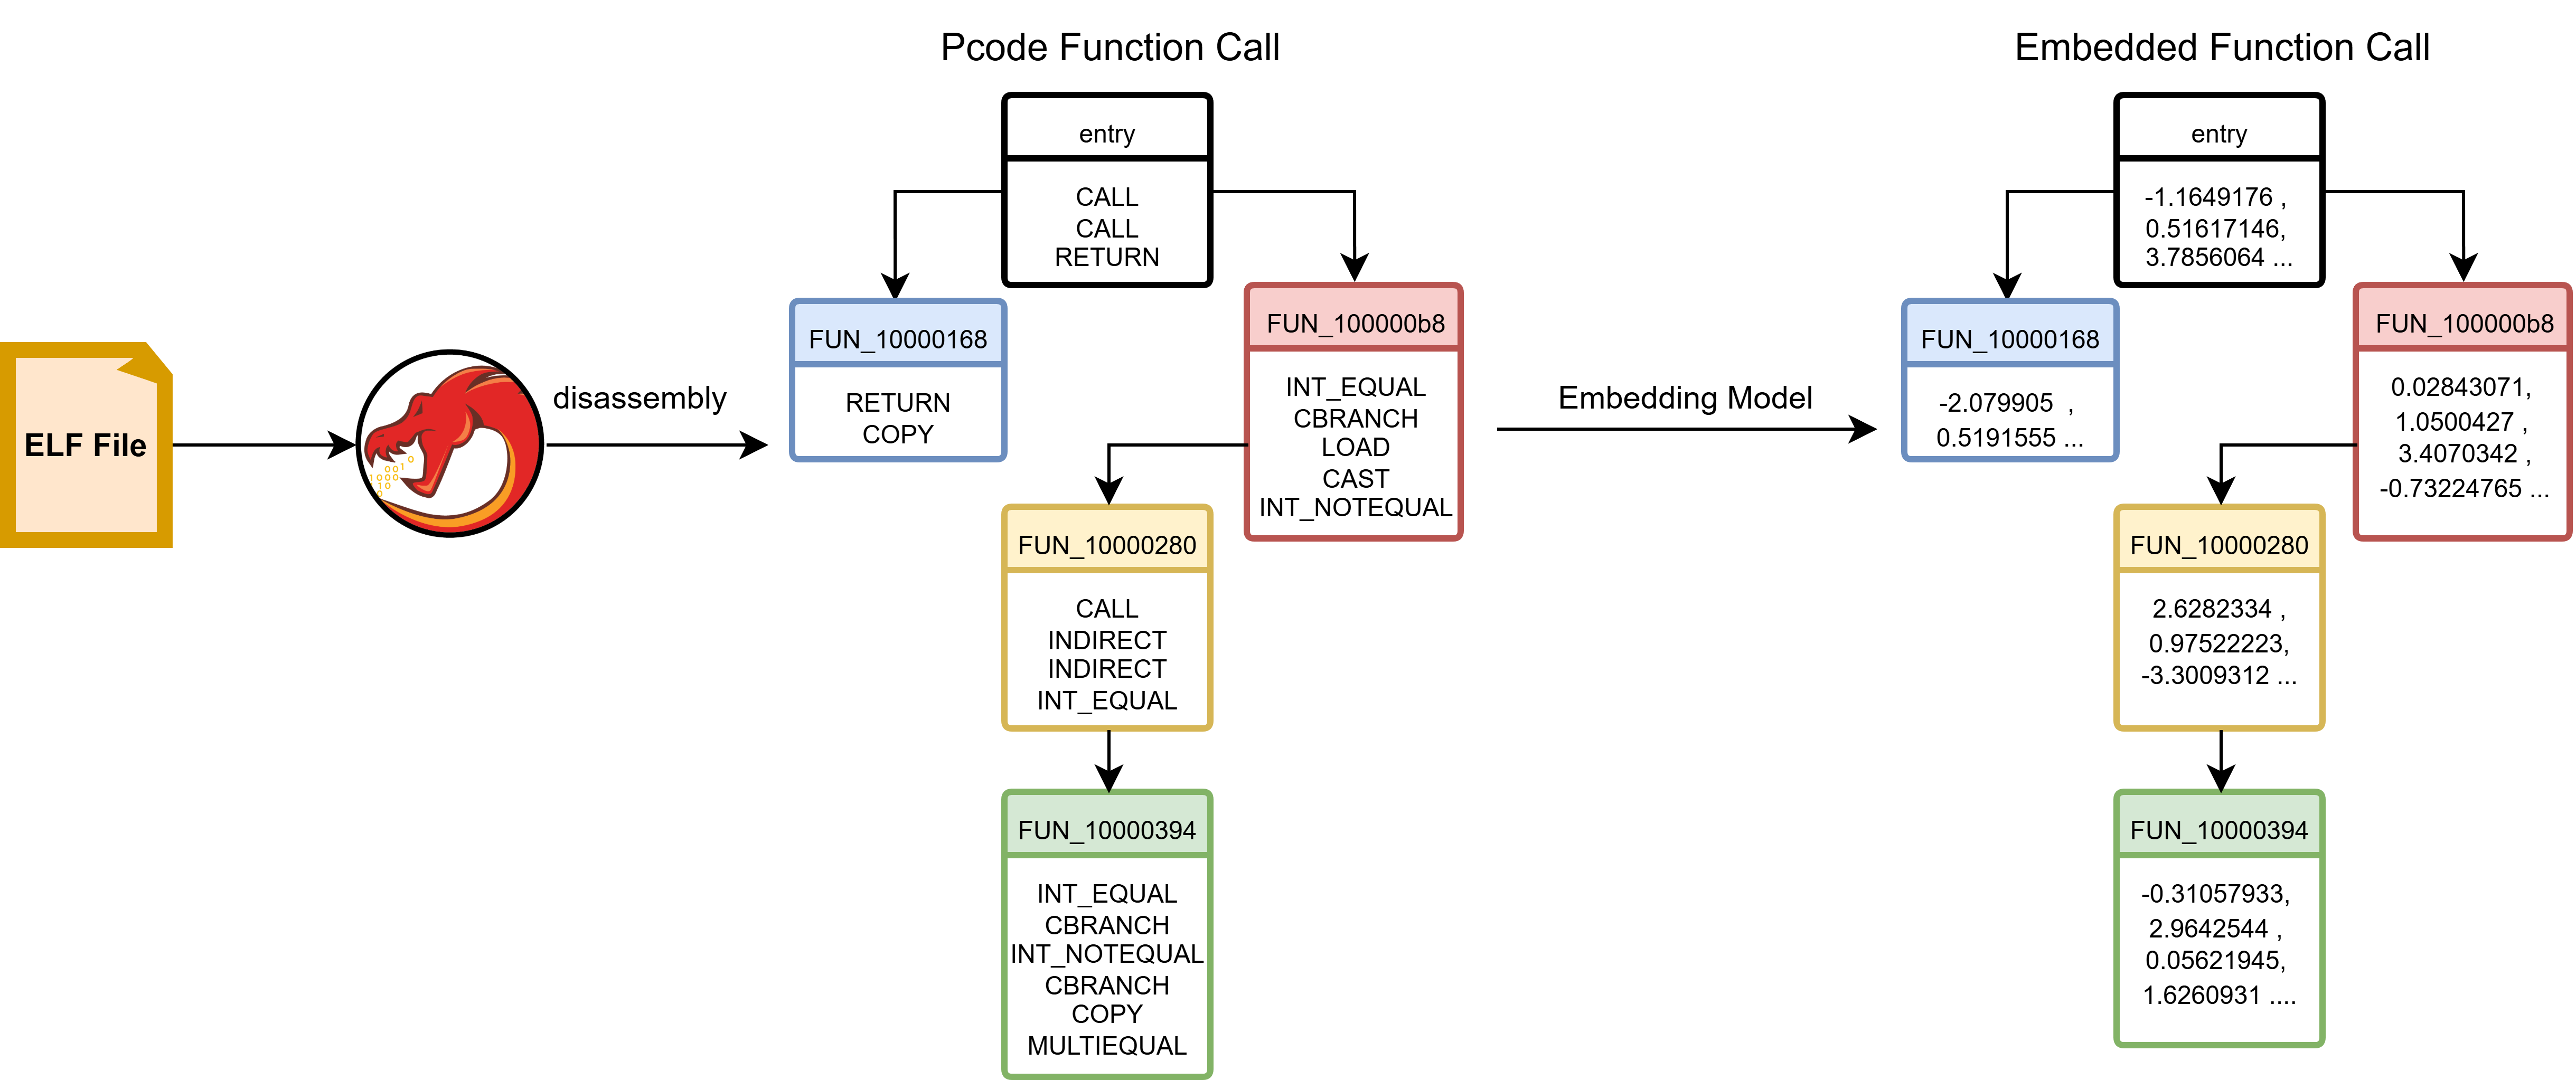
\includegraphics[width=\columnwidth]{fig/overview_feature_extraction.png}
\caption{特徵處理流程：從 ELF 二進制檔案經 Ghidra 轉換為函數呼叫圖，再進行圖嵌入。}
\label{fig:feature}
\end{figure}

\begin{figure*}[t]
\centering
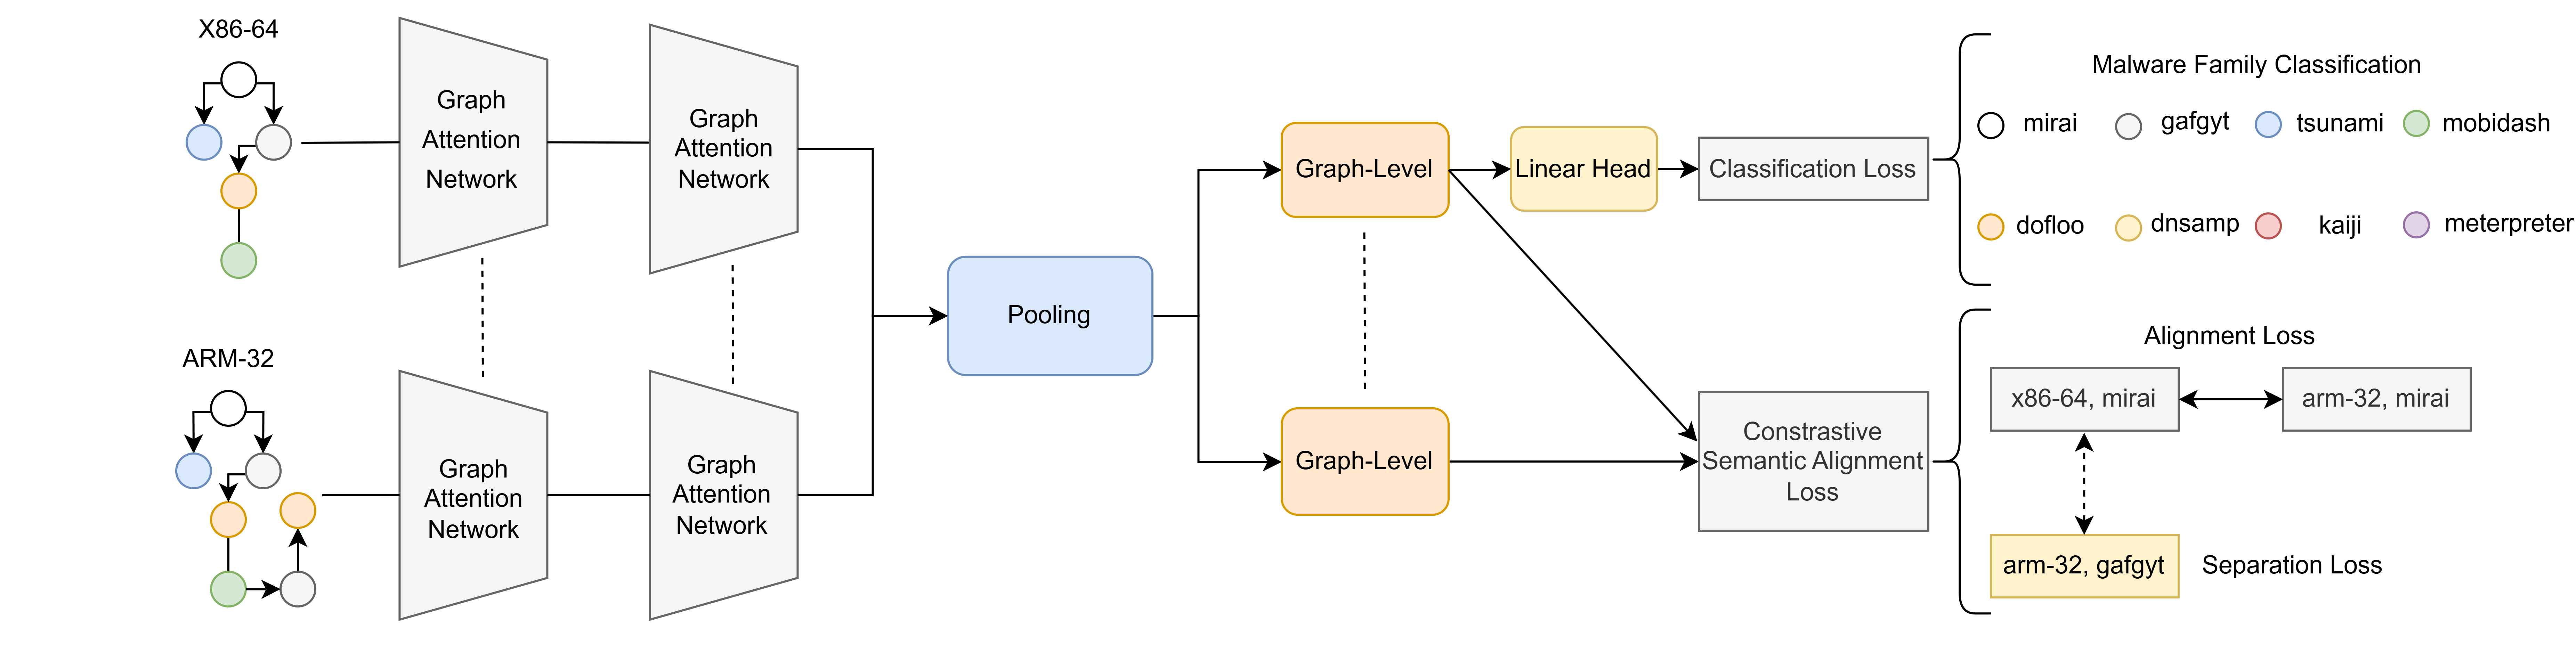
\includegraphics[width=\textwidth]{fig/overview.png}
\caption{所提跨架構惡意軟體偵測框架整體架構概覽。}
\label{fig:method}
\end{figure*}

% ============================
% 3.2 預訓練語言模型
% ============================
\subsection{預訓練語言模型}

本研究採用 RoBERTa~\cite{liu2019roberta} 對各函式節點的 P-Code 序列進行語意編碼。由於 P-Code 序列長度遠長於 Opcode 等特徵，RoBERTa 的 Transformer 架構能透過自注意力機制有效捕捉指令間的長程依賴，並以輕量架構從頭預訓練以適應 P-Code 領域語彙（詳細超參數設定於第 4.1 節）。

\textbf{Tokenizer.}~由於 P-Code 操作碼來自有限的指令集，本研究採用詞層級分詞（Word-level Tokenization），以空白字元為切分邊界，掃描訓練語料中所有唯一的 P-Code token 建立詞彙表，並加入 \texttt{[CLS]}、\texttt{[SEP]}、\texttt{[MASK]}、\texttt{[PAD]}、\texttt{[UNK]} 五個特殊 token。每條序列經 tokenizer 後，自動在首尾插入 \texttt{[CLS]} 與 \texttt{[SEP]}，再截斷或填補至最大長度 512。

給定函式節點 $v$ 對應的 P-Code token 序列 $\mathbf{x}_v = (t_1, t_2, \ldots, t_L)$，RoBERTa 輸出各位置的隱藏狀態（hidden state）$\{\mathbf{h}_1, \ldots, \mathbf{h}_L\}$，節點嵌入以 mean pooling 計算：
\begin{equation}
  \mathbf{e}_v = \frac{1}{L}\sum_{l=1}^{L} \mathbf{h}_l
\end{equation}

如圖~\ref{fig:mlm} 所示，本研究以 MLM 任務從頭預訓練。MLM 由 BERT~\cite{devlin2019bert} 所提出，對每條輸入序列隨機選取 15\% 的 token 位置構成遮蔽集合 $\mathcal{M}$；被選中的位置中，80\% 替換為 \texttt{[MASK]}，10\% 替換為詞彙表中的隨機 token，10\% 保持原 token 不變。訓練目標為最小化被遮蔽位置的交叉熵損失：
\begin{equation}
  \mathcal{L}_{\text{MLM}} = -\sum_{i \in \mathcal{M}} \log P(t_i \mid \mathbf{x}_{\setminus \mathcal{M}})
\end{equation}
其中 $\mathcal{M}$ 為被遮蔽位置之集合。各架構下超過 92\% 的函式節點 token 長度不超過 512，序列上限設為 512 可覆蓋絕大多數函式。

\begin{figure}[h]
\centering
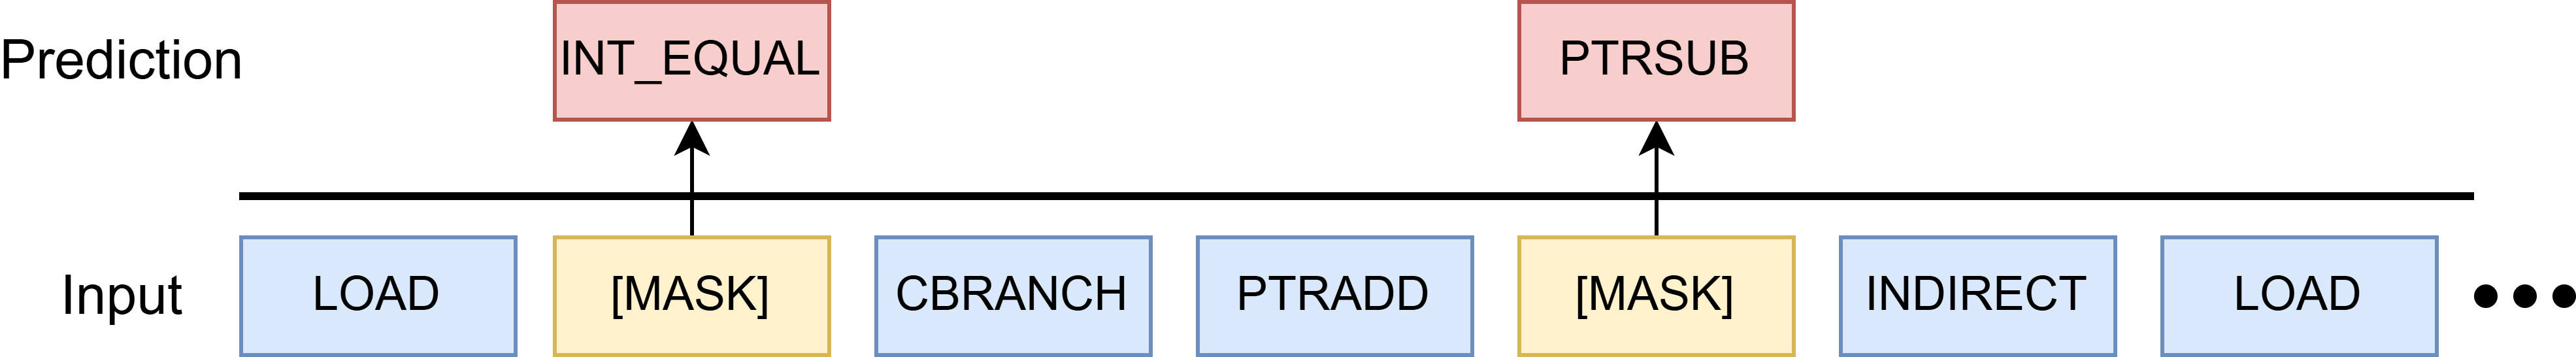
\includegraphics[width=\columnwidth]{fig/MLM.png}
\caption{以 MLM 任務預訓練：隨機遮蔽序列中的 P-Code後，訓練模型預測被遮蔽的 token，使模型學習 P-Code 序列的語意規律。}
\label{fig:mlm}
\end{figure}


% ============================
% 3.3 圖神經網路
% ============================
\subsection{圖神經網路}

本研究以 FCG 作為圖結構輸入，每個節點代表一個函式，初始節點特徵由 RoBERTa 所產生的嵌入 $\mathbf{e}_v$ 提供（即 $\mathbf{h}_v^{(0)} = \mathbf{e}_v$），函式間呼叫關係構成圖的邊集合 $\mathcal{E}$。本研究採用圖注意力網路（Graph Attention Network, GAT）~\cite{velivckovic2017graph} 對節點表示進行聚合，透過注意力機制自適應地加權鄰居貢獻。模型共設置 2 層：第一層使用 4 個注意力頭（multi-head attention）並將結果拼接輸出；第二層則使用單頭注意力，輸出維度 $d = 256$ 的最終節點表示 $\mathbf{h}_v^{(K)}$。

\textbf{注意力池化（Attentional Pooling）}~為將圖中所有節點表示聚合為固定維度的圖級嵌入（graph-level embedding），本研究採用注意力池化機制。對圖 $\mathcal{G}$ 中每個節點 $v$，以閘控網路（gate network）$f_{\text{gate}}$ 計算其重要性分數：
\begin{equation}
  e_v = f_{\text{gate}}(\mathbf{h}_v^{(K)}) = \mathbf{W}_2\,\mathrm{ReLU}(\mathbf{W}_1\,\mathbf{h}_v^{(K)})
\end{equation}
其中 $\mathbf{W}_1 \in \mathbb{R}^{128 \times 256}$、$\mathbf{W}_2 \in \mathbb{R}^{1 \times 128}$，接著以 softmax 正規化後加權加總所有節點表示：
\begin{equation}
  \mathbf{z} = \sum_{v \in \mathcal{G}} \frac{\exp(e_v)}{\sum_{u \in \mathcal{G}} \exp(e_u)}\, \mathbf{h}_v^{(K)}
\end{equation}
得到圖級嵌入 $\mathbf{z} \in \mathbb{R}^{256}$，作為後續分類與對比對齊的輸入。

\textbf{分類器}~圖級嵌入 $\mathbf{z}$ 輸入線性分類器 $\mathbf{W}_c \in \mathbb{R}^{|\mathcal{Y}| \times 256}$ 進行家族分類，輸出各類別的 logit，再以交叉熵損失 $\mathcal{L}_C$ 監督訓練。

% ============================
% 3.4 域適應與對比語意對齊
% ============================
\subsection{域適應與對比語意對齊}

跨架構泛化的核心挑戰在於協變量偏移（Covariate Shift）\cite{shimodaira2000improving}。第 2 節我們針對 P-Code 這個特徵的觀察，即使函式是一樣的原始碼，編譯至不同的指令集架構後，其 P-Code 序列與 FCG 特徵仍會產生顯著差異，導致源架構與目標架構的特徵邊際分佈並不相同（即 $P(\mathbf{X}^s) \neq P(\mathbf{X}^t)$）~\cite{blitzer2006domain}。本研究的直接遷移實驗（Lower Bound）進一步證實此偏移的影響：僅以源架構訓練的 GAT 模型會對其特徵分佈過擬合，導致映射至潛在空間的圖級嵌入仍帶有強烈的架構偏差（$P(\mathbf{Z}^s) \neq P(\mathbf{Z}^t)$），進而造成效能嚴重衰退。

為克服此特徵分佈差異，現有的無監督域適應（Unsupervised Domain Adaptation, UDA）方法通常透過對齊整體的機率分佈來進行特徵轉換~\cite{sun2016deep}。然而，文獻~\cite{motiian2017unified} 指出，若能進一步利用目標域中既有的少量標記樣本，則可引導模型實現更精確的類別層級對齊（Semantic Alignment）。基於此概念，本研究採用監督式域適應策略，引入並擴展 Motiian 等人提出的分類與對比語意對齊（CCSA）框架~\cite{motiian2017unified}，該框架最初在影像分類任務中取得成功，本研究將其應用至跨架構惡意軟體分析中，結合圖神經網路（GAT）提取圖級嵌入。此方法在目標架構僅有極少數標記的條件下，有效實現跨架構的語意對齊與特徵分離。

設 $\mathbf{z}^s_i$ 與 $\mathbf{z}^t_j$ 分別為源架構與目標架構樣本經 GAT 與注意力池化所得之圖級嵌入，於池化後施以 L2 正規化，$y^s_i$ 與 $y^t_j$ 為對應的家族標籤。定義正樣本對集合 $\mathcal{P} = \{(i,j) \mid y^s_i = y^t_j\}$ 與負樣本對集合 $\mathcal{N} = \{(i,j) \mid y^s_i \neq y^t_j\}$~\cite{hadsell2006dimensionality}。

語意對齊損失（Semantic Alignment Loss）縮短同家族跨架構嵌入之距離：
\begin{equation}
  \mathcal{L}_{\text{SA}} = \frac{1}{|\mathcal{P}|}\sum_{(i,j)\in\mathcal{P}} \|\mathbf{z}^s_i - \mathbf{z}^t_j\|^2
\end{equation}
類別分離損失（Separation Loss）對不同家族的跨架構嵌入施加 margin 懲罰：
\begin{equation}
  \mathcal{L}_{\text{Sep}} = \frac{1}{|\mathcal{N}|}\sum_{(i,j)\in\mathcal{N}} \max\!\left(0,\, m - \|\mathbf{z}^s_i - \mathbf{z}^t_j\|\right)^2
\end{equation}
其中 $m$ 為 margin 超參數，控制不同類別嵌入在空間中的最小分離程度。最終訓練目標結合分類損失 $\mathcal{L}_C$（交叉熵）與上述兩項對比對齊損失：
\begin{equation}
  \mathcal{L}_{\text{total}} = (1 - \alpha)\,\mathcal{L}_C + \alpha\,(\mathcal{L}_{\text{SA}} + \mathcal{L}_{\text{Sep}})
\end{equation}
其中 $\alpha \in [0,1]$ 平衡分類與對比對齊的比重。


% ============================
% 4. 實驗
% ============================
\section{實驗}

本節系統性地評估所提框架在單架構與跨架構場景下的性能。
% ============================
% 4.1 實驗設置
% ============================
\subsection{實驗設置}

實驗環境為配備 NVIDIA GeForce RTX 5070 Ti GPU 之工作站。

\textbf{預訓練語言模型（RoBERTa）：}採用 6 層 Transformer 架構，隱藏維度 256，8 個注意力頭，前饋層維度 1024，最大序列長度 512。以約 600 萬筆 x86\_64 架構函式節點之 P-Code 序列作為預訓練語料，以遮罩語言模型（MLM）任務從頭預訓練，遮罩比例 15\%，Adam 優化器，學習率 1e-4，Warmup 10,000 步，線性排程器，批次大小 64，訓練 100 個 epoch。

\textbf{GAT：}採用 2 層架構，隱藏維度 256，Dropout 0.2，注意力池化（Attention Pooling）。Adam 優化器，學習率 0.001，批次大小 32，最多訓練 200 個 epoch，Early Stopping（patience=15），損失函式為 Cross Entropy。

\textbf{CCSA：}以上述 GAT 架構為骨幹，加入對比語意對齊損失。損失權重 $\alpha = 0.3$，margin $m = 0.5$，目標域每類取 5 筆標記樣本（Few-shot），訓練時正負樣本對比例為 $1:3$。

\textbf{重複實驗：}單架構實驗與直接遷移（Lower Bound）因訓練與測試樣本固定，僅執行一次；跨架構實驗（Few-shot RF Baseline 與 Our Method）中，不同隨機種子會改變目標域 few-shot 訓練樣本、來源域訓練／驗證切割及測試樣本的組成，以 10 組不同隨機種子重複執行，並取 F1-macro 之平均值與標準差。


% ============================
% 4.2 資料集
% ============================
\subsection{資料集}

本研究收集涵蓋 ARM-32、ARM-64、Intel i386、MIPS、PowerPC（PPC）及 AMD x86-64 共六種架構之 IoT 惡意軟體樣本。所有樣本透過 VirusTotal\cite{virustotal2026} 進行多引擎掃描，並以 AVClass\cite{sebastianmilanesinovic2016avclass} 自動化工具統一標記惡意軟體家族，最終涵蓋十個家族，原始資料集共 36,078 個樣本。

在前處理階段，我們首先移除加殼樣本，因打包技術會掩蓋惡意軟體的固有特徵並扭曲分類結果；其次移除重複樣本，以防止訓練與測試階段之間發生資料洩漏。此外，部分二進位檔因逆向工程失敗而被排除：逾時（超過 600 秒）245 筆、節區格式錯誤 1,432 筆、無邊 1,017 筆、空節點 72 筆，共計移除 2,766 筆。最終有效資料集共 33,312 個樣本，各家族與架構之詳細分布如表~\ref{tab:dataset} 所示。

\begin{table*}[t]
\centering
\caption{實驗資料集各惡意軟體家族與架構之樣本數分布}
\label{tab:dataset}
\fontsize{8.5pt}{11pt}\selectfont
\begin{tabular}{lrrrrrrr}
\toprule
\textbf{Family} & \textbf{ARM-32} & \textbf{ARM-64} & \textbf{Intel} & \textbf{MIPS} & \textbf{PPC} & \textbf{x86\_64} & \textbf{Total} \\
\midrule
mirai       & 1,018 & 331 & 1,083 & 1,651 & 3,218 & 1,185 & 8,486 \\
gafgyt      & 1,054 &  20 & 1,094 & 1,715 & 3,214 & 1,203 & 8,300 \\
tsunami     &   983 &  25 & 1,095 & 1,683 &   530 & 1,206 & 5,522 \\
mobidash    & 1,063 & 284 & 1,098 &   306 &     0 & 1,216 & 3,967 \\
dofloo      & 1,062 &   0 & 1,095 &   365 &     0 &   129 & 2,651 \\
meterpreter &   137 &  46 &   598 &    47 &    24 & 1,154 & 2,006 \\
kaiji       &   134 &  91 &   211 &   164 &     0 &   244 &   844 \\
wroba       &   467 &  49 &   284 &     0 &     0 &     2 &   802 \\
dnsamp      &    95 &   0 &    99 &    64 &     0 &   208 &   466 \\
fakebank    &   217 &   0 &    51 &     0 &     0 &     0 &   268 \\
\midrule
\textbf{Total} & \textbf{6,230} & \textbf{846} & \textbf{6,708} & \textbf{5,995} & \textbf{6,986} & \textbf{6,547} & \textbf{33,312} \\
\bottomrule
\end{tabular}
\end{table*}

% ============================
% 4.3 實驗資料切割
% ============================
\subsection{實驗資料切割}

為確保各實驗具備可比較性，本研究針對單架構與跨架構兩種場景分別制定資料切割策略。由於 IoT 真實環境所蒐集之樣本在各架構與各家族之間分布高度不均（如表~\ref{tab:dataset}），部分家族在特定架構下樣本數極少，直接隨機切割將導致測試集過小而評估不具代表性。為此，我們採用以下統一切割原則：測試集每個家族各取約 50 個樣本；訓練集每個家族至多保留 300 個樣本。此一原則同時適用於單架構、跨架構與跨架構遷移學習三種實驗設置，確保三者採用相同的評量資料，具備公平可比較的基準。依此原則，最終納入實驗之樣本涵蓋 ARM-32、Intel、MIPS、x86\_64 共四種架構，以及 dnsamp、dofloo、gafgyt、kaiji、\allowbreak meterpreter、mirai、mobidash、tsunami 共八個惡意軟體家族。各家族在不同架構下之訓練樣本數介於 47 至 300 之間，樣本數充足之家族（如 gafgyt、mirai 等）各架構均達上限 300 筆，樣本較稀缺之家族（如 dnsamp、meterpreter）則取全部可用樣本。

% ============================
% 4.4 單架構分類
% ============================
\subsection{單架構分類}

單架構實驗目的在於建立各架構下的性能上界，確認模型在同架構訓練與測試時的分類能力。PLM（RoBERTa）以 x86\_64 架構資料進行預訓練；GAT 各自以當前架構之資料進行訓練與測試，採 60/20/20 之訓練、驗證、測試比例分割。各架構均可達 F1-macro 94\% 以上，驗證所提框架在同架構場景下具備穩定之分類能力。

% ============================
% 4.5 跨架構遷移學習比較
% ============================
\subsection{跨架構遷移學習比較}

表~\ref{tab:all-results} 整合單架構與跨架構各設定之 F1-macro，以統一評量指標進行比較，共四種設定：

\textbf{Upper Bound（單架構）}：Source 與 Target 為同一架構，代表理想情境下的性能上界。

\textbf{Lower Bound（跨架構 Source Only）}：GAT 以 Source 架構全量資料訓練，直接在 Target 架構測試，不進行任何適應，代表跨架構遷移之下界。

\textbf{Few-shot Baseline（RF）}：不使用 Source 資料，僅從 Target 架構每個家族取 5 筆樣本，對 GNN Embedding 做 Mean Pooling 後訓練 Random Forest（200 棵樹，\allowbreak max\_features=sqrt）。我們比較了 XGBoost、SVM 及 Random Forest 多種模型與參數組合，Random Forest 表現最佳，故以此為代表。

\textbf{Our Method（跨架構 + DA）}：在 Source 架構訓練基礎上，引入對比語意對齊域適應框架，利用 Target 架構每個家族 5 筆有標記樣本進行對齊微調。

\begin{table}[htbp]
\centering
\caption{單架構與跨架構各設定 F1-macro 比較（mean $\pm$ std）}
\label{tab:all-results}
\fontsize{7.5pt}{9.5pt}\selectfont
\setlength{\tabcolsep}{4pt}
\begin{tabular}{lcc}
\toprule
& \multicolumn{2}{c}{\textbf{F1-macro}} \\
\cmidrule(lr){2-3}
\multicolumn{1}{l}{\textbf{Architecture}} & \textbf{Upper Bound} & \textbf{Few-shot RF} \\
\midrule
ARM-32  & $0.9613 \pm 0.0095$ & $0.7978 \pm 0.0339$ \\
Intel   & $0.9781 \pm 0.0049$ & $0.8256 \pm 0.0365$ \\
MIPS    & $0.9448 \pm 0.0042$ & $0.8010 \pm 0.0375$ \\
x86\_64 & $0.9653 \pm 0.0154$ & $0.8163 \pm 0.0314$ \\
\midrule
\multicolumn{1}{l}{\textbf{Source $\rightarrow$ Target}} & \textbf{Lower Bound} & \textbf{Our Method} \\
\midrule
x86\_64 $\rightarrow$ ARM-32  & $0.4659$ & $\mathbf{0.9249 \pm 0.0156}$ \\
x86\_64 $\rightarrow$ Intel   & $0.8483$ & $\mathbf{0.9178 \pm 0.0040}$ \\
x86\_64 $\rightarrow$ MIPS    & $0.2228$ & $\mathbf{0.8806 \pm 0.0288}$ \\
ARM-32  $\rightarrow$ Intel   & $0.7800$ & $\mathbf{0.8916 \pm 0.0147}$ \\
ARM-32  $\rightarrow$ MIPS    & $0.5271$ & $\mathbf{0.9214 \pm 0.0295}$ \\
ARM-32  $\rightarrow$ x86\_64 & $0.6723$ & $\mathbf{0.8939 \pm 0.0061}$ \\
Intel   $\rightarrow$ ARM-32  & $0.6993$ & $\mathbf{0.9323 \pm 0.0104}$ \\
Intel   $\rightarrow$ MIPS    & $0.4398$ & $\mathbf{0.8915 \pm 0.0133}$ \\
Intel   $\rightarrow$ x86\_64 & $0.9185$ & $\mathbf{0.9491 \pm 0.0076}$ \\
\bottomrule
\end{tabular}
\end{table}

Upper Bound 各架構均達 F1 $>$ 0.94，確立性能上界。Lower Bound 代表分佈偏移的結果：x86\_64 直接測試於 MIPS 僅 0.2228，ARM-32 僅 0.4659。Few-shot Baseline 在不使用 Source 資料的條件下，僅以每類 5 筆樣本達 F1 約 0.80，可作為資料稀缺場景之基準。本研究之方法均達 F1 $\geq$ 0.88，最高為 Intel $\rightarrow$ x86\_64 之 0.9491，較各對應 Lower Bound 平均提升 0.29。


% ============================
% 5. 結論
% ============================
\section{結論}

本文提出一種以 Ghidra High P-Code 為統一中介表示之跨架構 IoT 惡意軟體分析框架，結合 RoBERTa PLM 與 GAT，同時建模 P-Code 指令序列之語意特徵與 FCG 之結構特徵。針對目標架構標記資料匱乏的挑戰，本研究引入監督式域適應機制，僅需每類 5 筆目標域樣本縮小跨架構特徵分佈差距。實驗結果顯示，單架構場景下各架構 F1-macro 均超過 94\%；跨架構場景下均達 0.88 以上，相較 Lower Bound 平均提升 0.29，最高提升 0.66。未來工作將探索更有效的嵌入空間對齊策略，並進一步分析跨架構嵌入空間之結構與可解釋性。


\bibliography{reference}
\bibliographystyle{abbrv}

\end{CJK*}
\end{document}

% 200620 lindawan https://github.com/lindawan/
